\documentclass{standalone}
\usepackage[subpreambles = true]{standalone}

\usepackage{tikz}
\usepackage{circuitikz}
\usetikzlibrary{patterns,decorations.pathmorphing,positioning}


\begin{document}
	
	\begin{figure*}[!htp]
		\begin{center}
			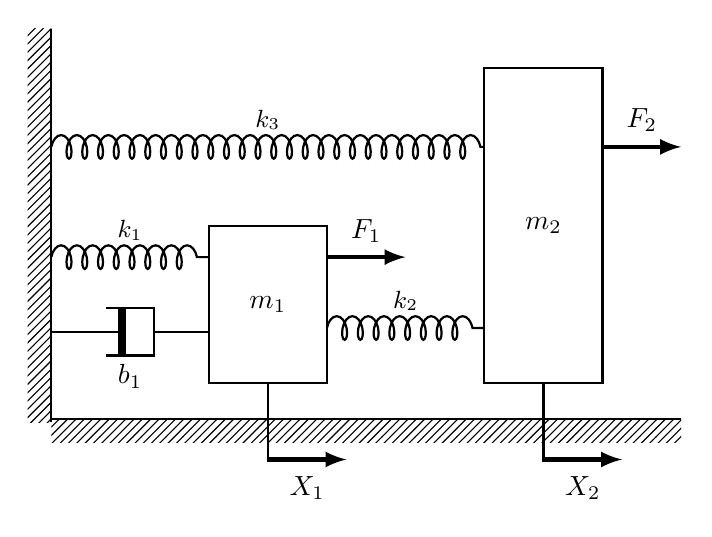
\begin{tikzpicture}[every node/.style={outer sep=0pt},thick,
 mass/.style={draw,thick},
 spring/.style={thick,decorate,decoration={zigzag,pre length=0.3cm,post
 length=0.3cm,segment length=6}},
 ground/.style={fill,pattern=north east lines,draw=none,minimum
 width=0.75cm,minimum height=0.3cm},
 dampic/.pic={\fill[white] (-0.1,-0.3) rectangle (0.3,0.3);
 \draw (-0.3,0.3) -| (0.3,-0.3) -- (-0.3,-0.3);
 \draw[line width=1mm] (-0.1,-0.3) -- (-0.1,0.3);}]
  \node[mass,minimum width=1.5cm,minimum height=2cm] (m1) {$m_1$} ;
  
  \node[mass,minimum width=1.5cm,minimum height=4cm,right=2cm of  m1, yshift = 1cm] (m2)  {$m_2$} ;
  
  
\node[left=-0.75cm of m1,minimum width=1.5mm,minimum height=1cm,yshift =-1.5cm] (l1){};
\draw (l1.north east) -- (l1.south east);
\draw [-latex,ultra thick] ([yshift=-0.47cm]l1.east)  -- +(1cm,0cm) node[midway,below=1mm] (x1) {$X_1$};

\node[left=-0.75cm of m2,minimum width=1.5mm,minimum height=1cm,yshift =-2.5cm] (l2){};
\draw (l2.north east) -- (l2.south east);
\draw [-latex,ultra thick] ([yshift=-0.47cm]l2.east)  -- +(1cm,0cm) node[midway,below=1mm] (x2) {$X_2$};



\node[left=2cm of m1,ground,minimum width=3mm,minimum height=5cm,yshift = 1cm] (g1){};
\draw (g1.north east) -- (g1.south east);


\node[right=-3.5cm of m1,ground,minimum width=8cm,minimum height=3mm,yshift = -1.6cm] (g2){};
\draw ([yshift=1.4mm]g2.west) -- ([yshift=1.4mm]g2.east);


 %\draw[spring] ([yshift=-0.40cm]g1.east) coordinate(aux) -- (m1.west|-aux) node[midway,above=1mm]{$k_1$};
 %\draw[spring] ([yshift=-3mm]m1.east) coordinate(aux) -- (m2.west|-aux) node[midway,above=1mm]{$k_2$};
 %\draw[spring] ([yshift=1cm]g1.east) coordinate(aux) -- (m2.west|-aux) node[midway,above=1mm]{$k_3$};
   
\draw[decoration={aspect=0.5, amplitude=1.5mm,segment length=2mm,coil},decorate] ([yshift=-0.40cm]g1.east) coordinate(aux) -- (m1.west|-aux) node[midway,above=1mm]{\small $k_1$};
\draw[decoration={aspect=0.5, amplitude=1.5mm,segment length=2mm,coil},decorate] ([yshift=-3mm]m1.east) coordinate(aux) -- (m2.west|-aux) node[midway,above=1mm]{\small $k_2$};
\draw[decoration={aspect=0.5, amplitude=1.5mm,segment length=2mm,coil},decorate] ([yshift=1cm]g1.east) coordinate(aux) -- (m2.west|-aux) node[midway,above=1mm]{\small $k_3$};


\draw [-latex,ultra thick] ([yshift=6mm]m1.east)  -- +(1cm,0cm) node[midway,below=-6mm] (F1) {$F_1$};
\draw [-latex,ultra thick] ([yshift=1cm]m2.east)  -- +(1cm,0cm) node[midway,below=-6mm] (F2) {$F_2$};

  \draw ([yshift=-1.35cm]g1.east) coordinate(aux')
   -- (m1.west|-aux') pic[midway]{dampic} node[midway,below=3mm]{$b_1$};
     %(m1.east|-aux') -- (m2.west|-aux') pic[midway]{dampic} node[midway,below=3mm]{$c_2$}
     %(m2.east|-aux') -- (ma.west|-aux') pic[midway]{dampic} node[midway,below=3mm]{$c_a$};

\tikzstyle{spring}=[thick,decorate,decoration={zigzag,pre length=0.1cm,post
  length=0.1cm,segment length=6}]
\end{tikzpicture}
		\end{center}
		\caption{Sơ đồ bài 1}
		\label{b1-diagram}
	\end{figure*}
	
	\section{Yêu cầu}%---------------------------------
	\begin{itemize}
		\item Xác định mô hình bài toán
		\item Mô phỏng bằng simulink
	\end{itemize}
	
	\section{Tính toán giá trị đề cho}%-------------------------
	\pagebreak
	\begin{table}[!htp]
		\centering
		\begin{tabular}{|l|l|l|}
			\hline $k_1$ = [1+2] & $k_2$ = [6] & $k_3$ = [3+1]\\
			\hline $m_1$ = 10[1+2] & $m_2$ = 10[1+3] & $b_1$ = [5]\\
			\hline
		\end{tabular}
		\caption{Bảng các thông số dựa trên MSSV bài 1}
		\label{b1-para-table}
	\end{table}
	Dựa vào bảng trên với MSSV là B1907058, ta dễ dàng tính được các thông số cần thiết như bảng sau:\\
	\begin{table}[!htp]
		\centering
		\begin{tabular}{|l|l|l|}
			\hline $k_1$ = 13 N/m & $k_2$ = 9 N/m & $k_3$ = 8 N/m\\
			\hline $m_1$ = 130 Kg & $m_2$ = 80 kg & $b_1$ = 0\\
			\hline
		\end{tabular}
		\caption{Bảng các thông số cần thiết bài 1}
		\label{b1-value-table}
	\end{table}
	
	\section{Tính mô hình bài toán}
	
	\subsection{Vật 1}%---------------------------------
	Ta chọn độ dịch chuyển của vật nặng theo tọa độ x:
	\vspace{1cm}
	\begin{figure*}[!htp]
		\centering
		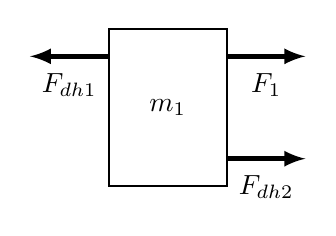
\begin{tikzpicture}[every node/.style={outer sep=0pt},thick,
 mass/.style={draw,thick},
 spring/.style={thick,decorate,decoration={zigzag,pre length=0.3cm,post
 length=0.3cm,segment length=6}},
 ground/.style={fill,pattern=north east lines,draw=none,minimum
 width=0.75cm,minimum height=0.3cm},
 dampic/.pic={\fill[white] (-0.1,-0.3) rectangle (0.3,0.3);
 \draw (-0.3,0.3) -| (0.3,-0.3) -- (-0.3,-0.3);
 \draw[line width=1mm] (-0.1,-0.3) -- (-0.1,0.3);}]


 
  
  \node[mass,minimum width=1.5cm,minimum height=2cm] (m2)  {$m_1$} ;
  
  
\draw [-latex,ultra thick] ([yshift=0.65cm]m2.east)  -- +(1cm,0cm) node[midway,below=1mm] (f1) {$F_1$};
\draw [-latex,ultra thick] ([yshift=-0.65cm]m2.east)  -- +(1cm,0cm) node[midway,below=1mm] (fdh2) {$F_{dh2}$};
\draw [-latex,ultra thick] ([yshift=0.65cm]m2.west)  -- +(-1cm,0cm) node[midway,below=1mm] (fdh1) {$F_{dh1}$};




\end{tikzpicture}
		\caption{Vật 1}
		\label{b1-vat-1}
	\end{figure*}\\
	Áp dụng định luật II Newton theo chiều x:
		\[ \sum F = ma,\]
		\[F_1 - k_1\,x_1 + k_2\,(x_2 - x_1) = m_1\,\ddot x_1\]\\
	Biểu diễn dạng chuẩn của mô hình toán:
	\[\ddot x_1 = \frac{1}{m_1}\,\left[F_1 - k_1\,x_1 + k_2\,(x_2 - x_1)\right]\]
	\[ \Rightarrow \ddot x_1 = \frac{1}{130}\,\left[F_1 - 13\,x_1 + 9\,(x_2 - x_1)\right] \]
	%\pagebreak
	\subsection{Vật 2}%-------------------------
	Ta chọn độ dịch chuyển của vật nặng theo tọa độ x:
	\vspace{1cm}
	\begin{figure*}[!htp]
		\centering
		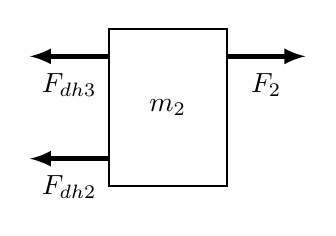
\begin{tikzpicture}[every node/.style={outer sep=0pt},thick,
 mass/.style={draw,thick},
 spring/.style={thick,decorate,decoration={zigzag,pre length=0.3cm,post
 length=0.3cm,segment length=6}},
 ground/.style={fill,pattern=north east lines,draw=none,minimum
 width=0.75cm,minimum height=0.3cm},
 dampic/.pic={\fill[white] (-0.1,-0.3) rectangle (0.3,0.3);
 \draw (-0.3,0.3) -| (0.3,-0.3) -- (-0.3,-0.3);
 \draw[line width=1mm] (-0.1,-0.3) -- (-0.1,0.3);}]


  \node[mass,minimum width=1.5cm,minimum height=2cm] (m1) {$m_2$};


\draw [-latex,ultra thick] ([yshift=0.65cm]m1.east)  -- +(1cm,0cm) node[midway,below=1mm] (f1) {$F_2$};
\draw [-latex,ultra thick] ([yshift=-0.65cm]m1.west)  -- +(-1cm,0cm) node[midway,below=1mm] (fdh2) {$F_{dh2}$};
\draw [-latex,ultra thick] ([yshift=0.65cm]m1.west)  -- +(-1cm,0cm) node[midway,below=1mm] (fdh1) {$F_{dh3}$};


\end{tikzpicture}

		\caption{Vật 2}
		\label{b1-vat-2}
	\end{figure*}\\
	Áp dụng định luật II Newton theo chiều x:
		\[ \sum F = ma,\]
		\[F_2 - k_3\,x_2 - k_2\,(x_2 - x_1) = m_2\,\ddot x_2\]\\
	Biểu diễn dạng chuẩn của mô hình toán:
	\[\ddot x_2 = \frac{1}{m_2}\,\left[F_2 - k_3\,x_2 - k_2\,(x_2 - x_1)\right] \]
	\[ \Rightarrow \ddot x_2 = \frac{1}{80}\,\left[F_2 - 8\,x_2 + 9\,(x_2 - x_1)\right] \]
	
	
	\section{Mô phỏng bằng simulink}%-------------------------
	\begin{figure*}[!htp]
		\centering
		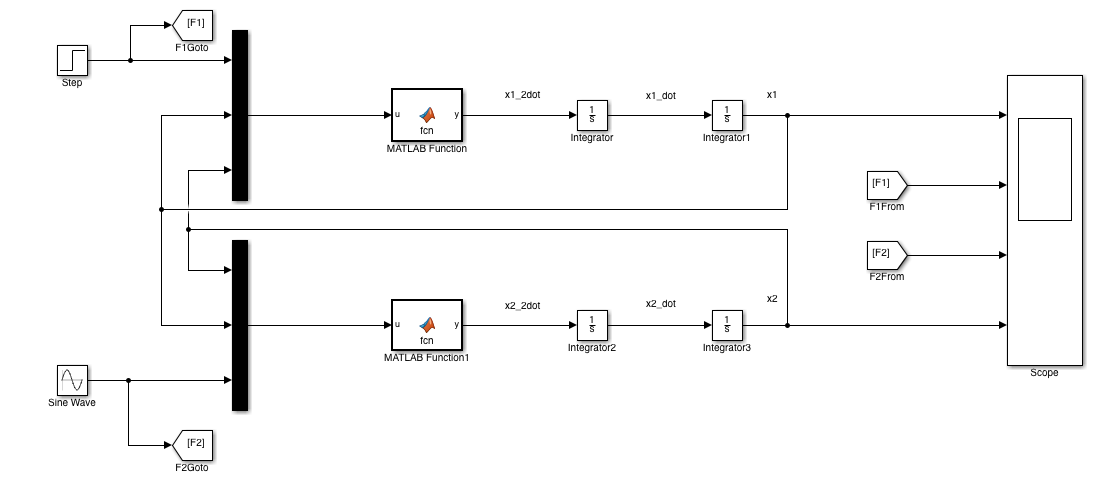
\includegraphics[scale=0.35]{images/b1-simu}
		\caption{Sơ đồ simulink bài 1}
		\label{b1-simu}
	\end{figure*}
	\pagebreak
	Với $F_1$ = u(t) trong đó u(t) là hàm step đơn vị, $F_2$ = $sin(\omega t)$.\\
	Giả sử các điều kiện đầu bằng 0. Các thông số được thấy từ bảng \ref{b1-value-table} ở trang \pageref{b1-value-table}.\\
	\begin{figure*}[!htp]
		\centering
		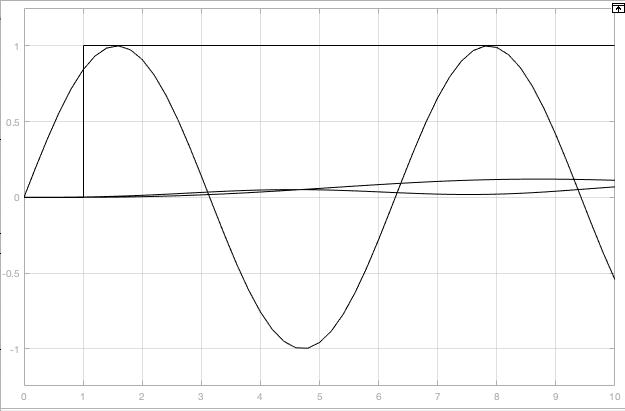
\includegraphics[scale=0.5]{images/b1-scop}
		\caption{Kết quả mô phỏng trên Oscilloscope bài 1}
		\label{b1-scop}
	\end{figure*}
	
	
	
	
	
\end{document}